\section{Dynamic model}
The Castle Creations ESC incorporates a microcontroller that employs a non-linear scaling mechanism to transform the input PWM signal's duty cycle ($u_p$) into the duty cycle of the $24,kHz$ PWM signals sent to the inverter, thereby effectively adjusting the source voltage applied to the motor\cite{kim2017electric}. This non-linear transformation aims to achieve a linear input-to-thrust relationship, departing from the quadratic one. Consequently, the PWM input to the ESC ($u_p$) undergoes filtering through a non-linear function, denoted as $g_m$, resulting in the PWM duty-cycle input to the inverter ($u_m$). This relationship can be represented as:
%===
\begin{align}\label{eqn::esc_input}
    u_m &= g_m(u_p)\quad
    V_s = u_m V_{in} \qquad u_m \in [0, 1]
\end{align}
\begin{align*}
\text{Where,}\qquad&\\
    V_s &- \text{Effective voltage to the motor (lumped)}\\
    V_{in} &- \text{Battery voltage}
\end{align*}
%===
A constant PWM switching frequency of $400 , Hz$ is utilized, and the duty cycle is scaled accordingly with this frequency. Notably, the current ESC equipped with RPM feedback capabilities operates within the range of $1110 , \mu s$ to $1890 , \mu s$. Beyond this range, the ESC switches to a constant power mode, maintaining a constant RPM.

It's worth noting that the specific parameters governing the non-linear filter are not ascertainable with the available information. Consequently, neither $u_m$ nor $u_p$ can be considered the true input for system identification in conjunction with the propeller. To circumvent this issue, we redefine the input as the motor's angular velocity with the propeller, normalized by the input voltage ($u_\omega$). We then establish a static mapping between this quantity and the PWM input to the ESC ($u_p$).


We have speed-torque characteristics of a BLDC motor \cite{crowder2019electric}:
%===
\begin{align}
    T_e &= K_T I = K_T \frac{(V_s - E)}{R} = \frac{K_T}{R} (V_s - K_v \omega)
\end{align}
Where,
\begin{align*}
    \omega &- \text{Mechanical rpm} & &
    T_e      - \text{Electromagnetic torque}\\
    E        &- \text{Back emf} & &
    V_s      - \text{Supply voltage}\\
    I        &- \text{Total DC current}& &
    R        - \text{Total terminal phase resistance}\\
    K_T      &- \text{Motor torque constant} & &
    K_v      - \text{Kv value of the motor= $K_T$}
\end{align*}
%===
Let, $K_r = \frac{K_T}{R}$.
From (\ref{eqn::esc_input}), we have the electromagnetic torque as a function
of input and rpm:
\begin{align}\label{eqn::Te}
    T_e &= u_m K_r V_{in} - K_r K_v \omega
\end{align}
%===
We use the following quadratic relationship between propeller aerodynamic forces
and RPM \cite{pounds2010modelling}:
\begin{align}
    &\text{Propeller Thrust:}\quad
    F_T = C_{T} \omega^2\\
    &\text{Propeller moment due to drag:}\quad
    M_D = C_{D} \omega^2
\end{align}
%===
In our system, with the motor operating in a single direction, we consider
Coulomb friction as $M_f$ and damping due to viscous friction as $b_f\omega$.
We have the dynamic model of the BLDC motor with propeller using moment balance:
%===
\begin{align}
    J \dot \omega &= T_e - b_f \omega - M_f - C_D \omega^2
\end{align}
Where, $J$ is the moment of inertia. Also, let $b_m = b_f + K_rK_v$. We have the dynamic model:
\begin{equation}\label{eqn::dyn_mdl}
    J\dot \omega + b_m \omega + C_D \omega^2 + M_f = u_m K_r V_{in}
\end{equation}
%===
\subsection{Normalized Angular Velocity Input}
In the steady-state condition ($\dot \omega = 0$), (\ref{eqn::dyn_mdl}) simplifies to:
%===
\begin{align}
    &\frac{b_m}{K_r} \left(\frac{\omega_m}{V_{in}}\right) + \frac{V_{in}}{K_r} C_D \lr{\frac{\omega}{V_{in}}}^2 + \frac{M_f}{K_r V_{in}} = u_m
\end{align}
%===
We introduce a term, $u_{\omega}$, which represents the angular velocity of the motor with the propeller at unit supply voltage for the given PWM input ($u_p$). This is termed as "\textit{Normalized Angular Velocity}".
%===
\begin{align}
    u_{\omega} &= \frac{\omega}{V_{in}} \text{  at  } u_m = g_m(u_p) \\
    %===
    \implies u_m &= \underbrace{\frac{b_m}{K_r} u_\omega + \frac{\hat V_{in}}{K_r} C_D u_\omega^2 + \frac{M_f}{K_r  \hat V_{in}}}_{g_\omega (u_\omega, \hat V_{in})}
     \label{eqn::input_def}
\end{align}
where $\hat V_{in}$ is the battery voltage at calibration $(15.54\,V)$.
%===
The relationship between $u_\omega$ and $u_p$ can be estimated from the static
measurement data (Fig.-\ref{fig::norm_omega}).
%===
\begin{figure}[h]
    \centering
    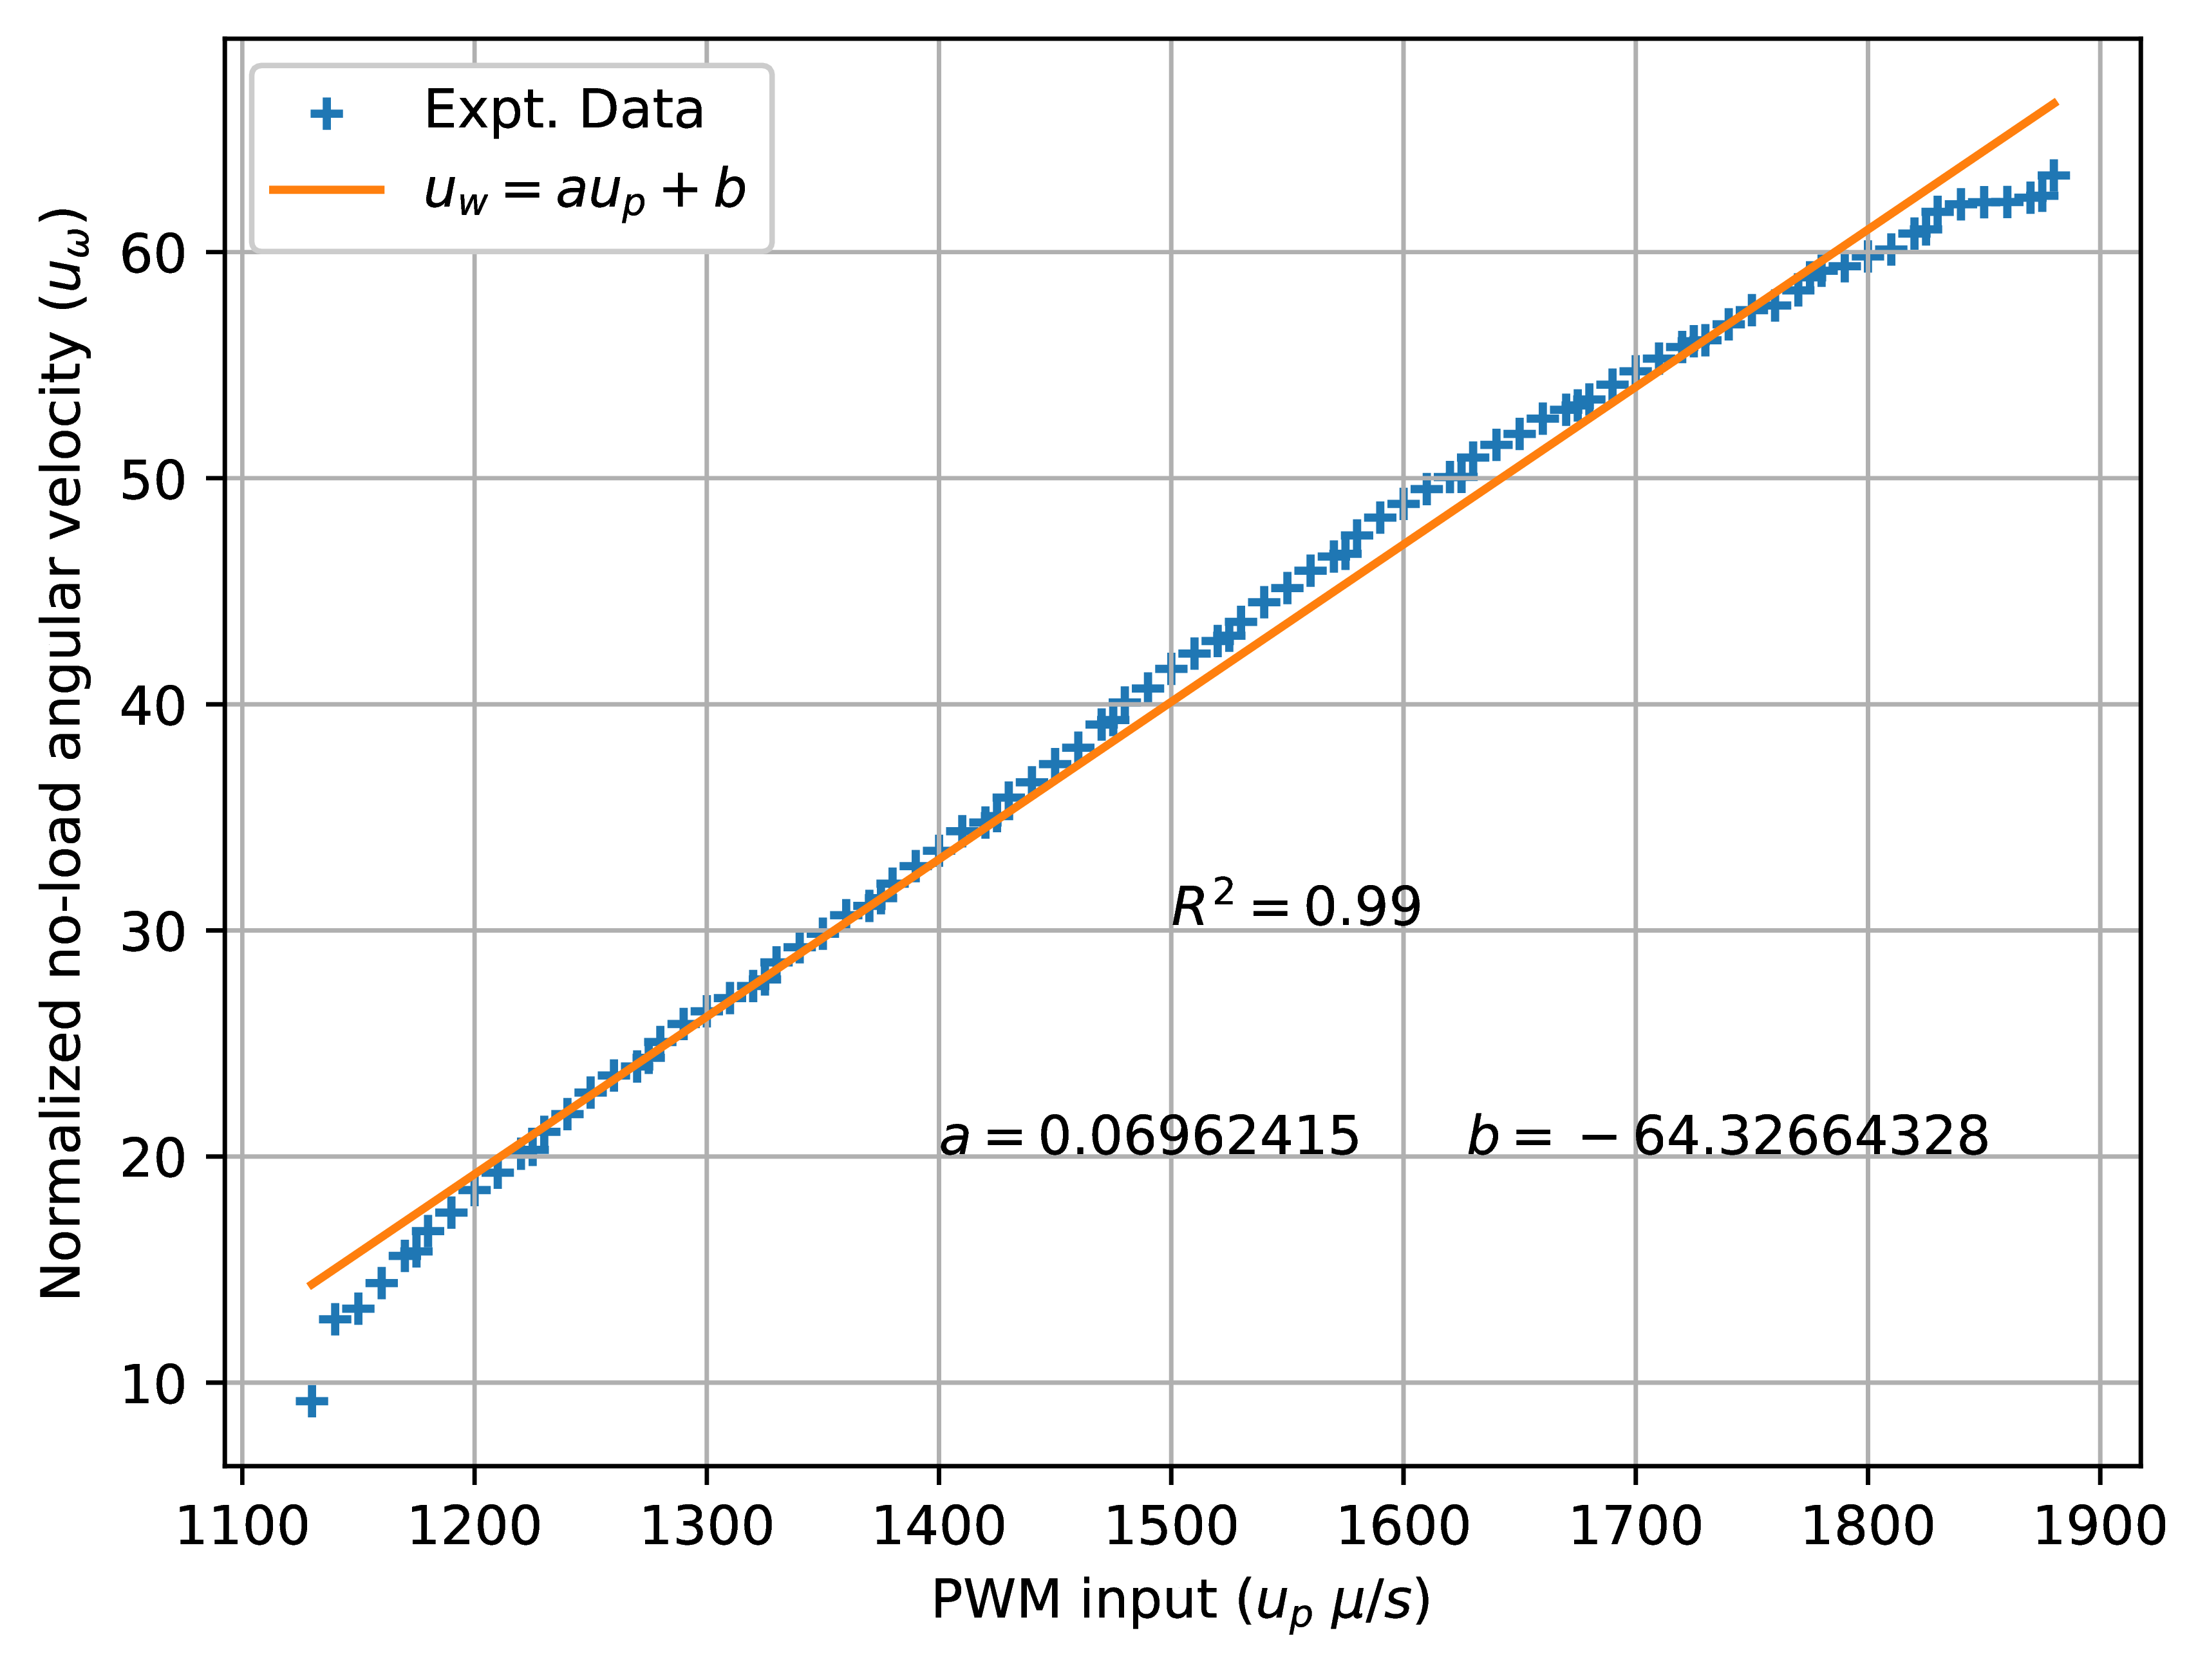
\includegraphics[width = \figsize]{./figs/figs_acc/norm_omega/no-load_rpm.png}
    \caption{$u_\omega$ as a function of $u_p$}
    \label{fig::norm_omega}
\end{figure}
%===
\begin{align}
    &u_\omega = a u_p + b
    \quad a = 0.0696
    \quad b = -64.3266   \label{eqn::uw_calib}\\
    \implies& g_m(u_p) = g_\omega(a u_p  + b, \hat V_{in})
    \; [\because u_m = g_\omega(u_\omega, \hat V_{in})]
\end{align}

%===
\subsection{Input-Output Model for Identification}
Incorporating the input definition (\ref{eqn::input_def}) into the BLDC motor model with the propeller (\ref{eqn:dyn_mdl}), we have:
%===
{\small
\begin{align}
    &J \dot \omega + b_m \omega + C_D \omega^2 + M_f \lr{1 - \frac{V_{in}}{\hat V_{in}}} = V_{in} b_m u_\omega + V_{in} \hat V_{in} C_D u_\omega^2
    \label{eqn::calib_mdl}
\end{align}
}
%===
We assume that the battery voltage remains approximately constant with small variations, which can be introduced as uncertainties:
%===
\begin{align}
    \hat V_{in} &= V_{in} ( 1 + \delta v)
    %\implies \frac{V_{in}}{\hat V_{in}} = 1 - \delta v\\
    \implies \lr{1 - \frac{V_{in}}{\hat V_{in}}} = \delta v
\end{align}
%====
This leads us to the following nonlinear input-output model with uncertainties:
\begin{equation}\label{eqn::nl_model}
    J \dot \omega + b_m \omega + C_D \omega^2 + M_f \delta v = V_{in} b_m u_\omega + V_{in}^2 (1 + \delta v) C_D u_\omega^2
\end{equation}
%===============================================================================

%===
\subsection{Model Parameter Estimates}
The model parameters and their variances are estimated using a combination of static experimental data and dynamic responses obtained under small-perturbation conditions. Subsequently, the resulting model is validated against the dynamic response of the full nonlinear model.
%===
\begin{table}[h]
    \centering
    \begin{tabular}{c l l c}
        \hline \hline
        Parameter & Value & Units & Variance ($\sigma$)            \\ \hline \hline
        $C_T$ & $7.2581 \times 10^{-06}$ & $N/(rad/s)^2$   & $4.4522 \times 10^{-8}$ \\
        $C_D$ & $3.6088 \times 10^{-08}$ & $N.m/(rad/s)^2$ & $1.3964 \times 10^{-9}$ \\
        $b_m$ & $0.0$                    & $N.m/(rad/s)$   & $4.6003 \times 10^{-6}$  \\
        $M_f$ & $1.3135 \times 10^{-3}$  & $N.m$           & $4.5277 \times 10^{-3}$ \\
        $J$   & $3.2238 \times 10^{-6}$   & $Kg.m^2$        & $7.0053 \times 10^{-6}$ \\
        \hline \hline
    \end{tabular}
    \caption{Summary of parameter estimates from static and small-perturbation experiments}
    \label{tab::parm_ests}
\end{table}

The bounds on the voltage variation based on the hard cut-off of the ESC
are found to be:
%===
\begin{align}
\abs{\delta v}_{max} = 0.2
\end{align}

Moreover, from the experiments the system start only at $u_\omega = 12.93$ which
is the minimum input required to overcome the static friction. This can be
verified as:
\begin{align}
     \lr{V_{in}^2  C_D u_\omega^2 }_{\lr{u_\omega = 12.93, V_{in} = 15.54}} = 1.4570 =  M_f
\end{align}

Thus, expanding the range of $u_w$ from $[12.93, 67.23]$ to $[0, 67.23]$, the
dynamic model \ref{eqn::nl_model} will now include the actual friction instead
of $\delta v M_f$. Rewriting \ref{eqn::calib_mdl}:

\begin{align}
    &J \dot \omega + b_m \omega + C_D \omega^2 + M_f = V_{in} \lr{b_m u_\omega + \hat V_{in} C_D u_\omega^2}
    \label{eqn::0_mdl}
\end{align}

%===
\subsection{Control form of the model}

Defining input to the system (u) as:
\begin{align}
    u &= \underbrace{\hat b_m u_\omega + \hat V_{in} \hat C_D u_\omega}_{g_u(u_\omega)} \label{eqn::uw2u}\\
    \implies u &= K_r u_m \qquad [\therefore u \geq 0] \label{eqn::ctrl_u}
\end{align}
Where $\hat \bullet$ are the estimated values of the parameters at the time of calibration.

Thus, $u$ is the actual PWM input to the inverter scaled by the ratio of the
torque constant and the winding resistance of the motor $\lr{\because K_r =
\frac{K_T}{R}}$.

Introducing the input definition (\ref{eqn::ctrl_u}) in to the nonlinear model
of the system (\ref{eqn::dyn_mdl}):
\begin{align*}
    J\dot \omega &+ b_m \omega + C_D \omega^2 + M_f = V_{in} u\\
    \implies \dot \omega  &= -\frac{b_m}{J} \omega - \frac{C_D}{J} \omega^2 - \frac{M_f}{J} + \frac{V_{in}}{J} u\\
\end{align*}
Introducing the input uncertainties as $\Delta(u, \omega, t)$ (matched). Let,
$\bullet_{_J} = \frac{\bullet}{J}$. We have the control form of the model:

\begin{align}
   \dot \omega &= -b_{m_J} \omega - C_{D_J} \omega^2 - M_{f_J} + V_{in_J} u + \Delta(t, u, \omega) \label{eqn::ctrl_form}
\end{align}

\subsubsection{Input uncertainties}
The uncertainties in the input arise from the changes in the voltage from
calibration and the real system, the uncertainties in the parameter estimation
and higher-order input dynamics if any.

\subsubsection{Input to the hardware}
The control input calculated from the algorithm is not the actual hardware
input rather a nonlinear injective function of the hardware input. The
uniqueness in the mapping comes from the constraints in the range of input
values $(u > 0)$. From (\ref{eqn::uw2u}):
\begin{align*}
    &\hat V_{in}^2 \hat C_D u_{\omega}^2 + \hat b_m u_\omega - u = 0\\
    %===
    \implies& u^{\pm}_\omega = \frac{-\hat b_m \pm \sqrt{\hat b_m ^2 + 4u \hat V_{in}^2 C_D}}{2 \hat V_{in}^2 C_D}\\
    %===
    \because \hat b_m, \hat C_D, \hat V_{in} &> 0 \quad \text{we have, }\qquad \\
    \implies& u^{+}_\omega = \frac{-\hat b_m + \sqrt{\hat b_m ^2 + 4u \hat V_{in}^2 C_D}}{2 \hat V_{in}^2 C_D} \geq 0 \quad \text{and} \quad
    u^{-}_\omega = \frac{-\hat b_m - \sqrt{\hat b_m ^2 + 4u \hat V_{in}^2 C_D}}{2 \hat V_{in}^2 C_D} \leq 0 \quad \
    \forall \; u \geq 0 \\
\end{align*}
As $u_\omega > 0$ we have a unique mapping from $u$ to $u_w$:
\begin{align}
    u_\omega &= \underbrace{\frac{-\hat b_m + \sqrt{\hat b_m ^2 + 4u \hat V_{in}^2 C_D}}{2 \hat V_{in}^2 C_D}}_{g_u^+(u)}
    \label{eqn::u2uw}\\
    \implies u_p &= \frac{1}{a} \lr{g_u^+(u) - b} \qquad [\because u_\omega = a u_p + b \quad (\ref{eqn::uw_calib})]
\end{align}

